\renewcommand*{\arraystretch}{1.1}

\subsection*{BI / read / 4}
\label{sec:bi-read-04}

\noindent\begin{tabularx}{\queryCardWidth}{|>{\queryPropertyCell}p{\queryPropertyCellWidth}|X|}
	\hline
	query & BI / read / 4 \\ \hline
%
	title & Popular topics in a country \\ \hline
%
	pattern & \hfill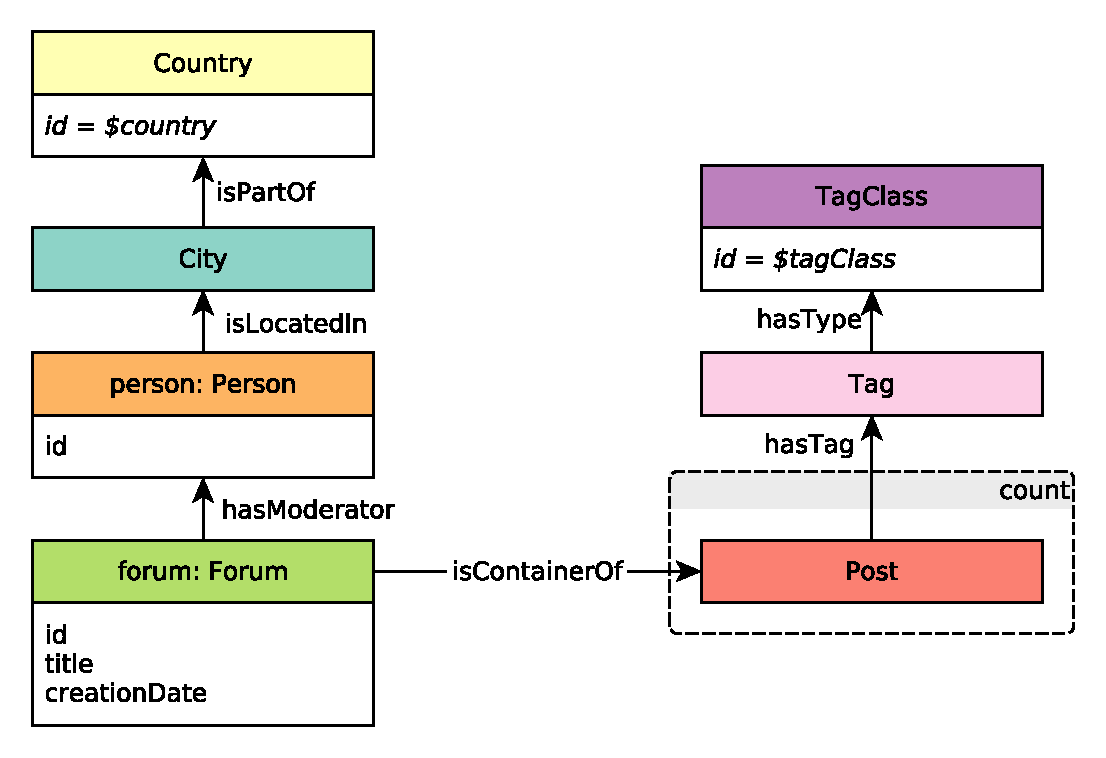
\includegraphics[scale=\patternscale,margin=0cm .2cm]{patterns/bi-read-04}\hfill\vadjust{} \\ \hline
%
	desc. & Given a TagClass and a Country, find all the Forums created in the given
Country, containing at least one Post with Tags belonging directly to
the given TagClass.

The location of a Forum is identified by the location of the Forum's
moderator.
 \\ \hline
%
	
%
	
		params &
		\innerCardVSpace{\begin{tabularx}{\attributeCardWidth}{|>{\paramNumberCell}c|>{\varNameCell}M|>{\typeCell}m{\typeWidth}|Y|} \hline
		$\mathsf{1}$ & tagClass & 32-bit Integer &  \\ \hline
		$\mathsf{2}$ & country & 32-bit Integer &  \\ \hline
		\end{tabularx}}\innerCardVSpace \\ \hline
	
%
	
		result &
		\innerCardVSpace{\begin{tabularx}{\attributeCardWidth}{|>{\resultNumberCell}c|>{\varNameCell}M|>{\typeCell}m{\typeWidth}|>{\resultOriginCell}c|Y|} \hline
		$\mathsf{1}$ & forum.id & 64-bit Integer & R &
				 \\ \hline
		$\mathsf{2}$ & forum.title & String & R &
				 \\ \hline
		$\mathsf{3}$ & forum.creationDate & DateTime & R &
				 \\ \hline
		$\mathsf{4}$ & person.id & 64-bit Integer & R &
				 \\ \hline
		$\mathsf{5}$ & postCount & 32-bit Integer & A &
				 \\ \hline
		\end{tabularx}}\innerCardVSpace \\ \hline
	
%
	
		sort		&
		\innerCardVSpace{\begin{tabular}{|>{\sortNumberCell}c|>{\varNameCell}l|>{\directionCell}c|} \hline
		$\mathsf{1}$ & count & $\desc$ \\ \hline
		$\mathsf{2}$ & forum.id & $\asc$ \\ \hline
		\end{tabular}}\innerCardVSpace \\ \hline
	%
	limit & 20 \\ \hline
	%
	CPs &
	\multicolumn{1}{>{\raggedright}l|}{
		\chokePoint{1.1}, 
		\chokePoint{1.2}, 
		\chokePoint{1.4}, 
		\chokePoint{2.1}, 
		\chokePoint{2.2}, 
		\chokePoint{2.4}, 
		\chokePoint{3.3}
		} \\ \hline
	%
	%
\end{tabularx}
\queryCardVSpace